\documentclass[12pt]{article}
\usepackage{geometry}                % See geometry.pdf to learn the layout options. There are lots.
\geometry{letterpaper}                   % ... or a4paper or a5paper or ... 
%\geometry{landscape}                % Activate for for rotated page geometry
\usepackage[parfill]{parskip}    % Activate to begin paragraphs with an empty line rather than an indent
\usepackage{daves,fancyhdr,natbib,graphicx,dcolumn,amsmath,lastpage,url}
\usepackage{amsmath,amssymb,epstopdf,longtable}
\DeclareGraphicsRule{.tif}{png}{.png}{`convert #1 `dirname #1`/`basename #1 .tif`.png}
\pagestyle{fancy}
\lhead{CE 3372 -- Water Systems Design}
\rhead{FALL 2020}
\lfoot{EXERCISE 1}
\cfoot{}
\rfoot{Page \thepage\ of \pageref{LastPage}}
\renewcommand\headrulewidth{0pt}


\begin{document}
\begin{center}
{\textbf{{ CE 3372 -- Water Systems Design} \\ {Exercise Set 1}}}
\end{center}

\section*{\small{Topographic/Contour Maps}}

Figure \ref{fig:somewhereUSABaseMap} is a subdivision conceptual map for Somewhere, USA.
The numbers on the map are land surface elevations located at the decimal points in the drawing.
Along the bottom edge of the map is a black line segment (with arrowheads at each end) that indicates a distance of 1,100 feet on the map. The black circle in the lower left hand corner is to be used as an origin for X-Y measurements for making XYZ data files.

\begin{figure}[h!] %  figure placement: here, top, bottom, or page
   \centering
   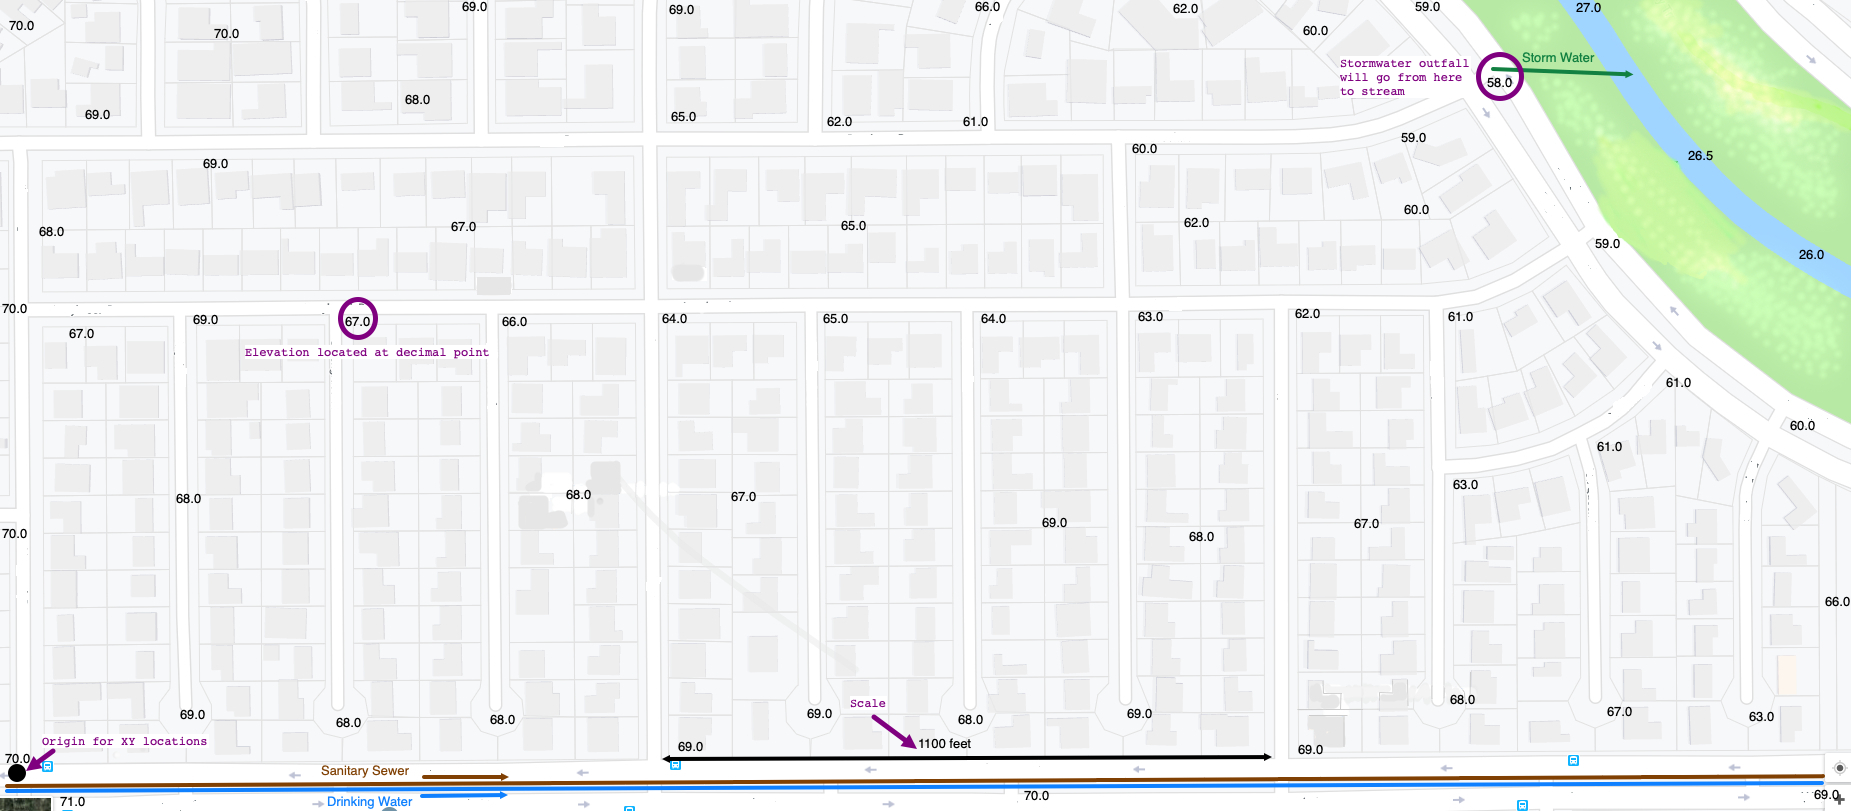
\includegraphics[width=6.5in]{SomewhereUSABaseMap.png} 
   \caption{Somewhere USA Study Area}
   \label{fig:somewhereUSABaseMap}
\end{figure}

You will be tasked with conceptual design of a water distribution, stormwater collection, and wastewater collection system for this subdivision.
All three systems will be influenced by the local topography, so a first step is to build a topographic map to guide design decisions, especially for the stormwater part of the design.  The \texttt{.png} file is included with the exercise so you can render a larger graphic if needed.

\section*{\small{Exercise}}
Construct a topographic contour map of the area.
\begin{enumerate}
\item Use the indicated origin and find X,Y, and Z coordinates for each displayed elevation. (50 points)
\item Arrange those coordinates into an ASCII (text) file where each row of the file is a coordinate triple. (10 points)
\item You can choose a variety of software to make a topographic map, even the class server can render a topographic contour map (20 points)
\item Use graphics tools to overlay the topographic map onto the base map (this is tricky, you will have to read how to make a layer have transparent portions to do the overlay, scaling and alignment take some effort) (20 points)
\end{enumerate}

Submit your completed map as a PDF file to Blackboard.
%Demand nodes are shown with the land surface elevations at the node locations and the
%population served by that particular node. The ductile iron pipes are shown with their
%length and nominal inside diameter.
%
%Figure 2 is a layout of a water distribution system for the subdivision. The blue line segments
%are pipes and are labeled (P1, P2, : : : ). The blue circles are nodes and are labeled (N1, N2,
%: : : ). The yellow polygons represent the demand lots assigned to each node. For example,
%node N2 supplies the six (6) individual lots located near the node.

%Figure \ref{fig:aerial} is an older (circa 1993) aerial image of a portion of Houston, Texas.   
%The red polygon is the drainage boundary for a storm sewer system that drains North from the part of the area near Westheimer Road to a tributary of Buffalo Bayou and East from the area.
%The drainage ditch is shown as the ``blue''   fuzzy line on the figure.  
%Drainage in the ditch is from West to East.
%The two main streets in the study area are highlighted in magenta.  
%\begin{figure}[h!] %  figure placement: here, top, bottom, or page
%   \centering
%   \includegraphics[height=5in]{Image118.jpg} 
%   \caption{Tanglewilde Drive Study Area}
%   \label{fig:aerial}
%\end{figure}
%\clearpage
%
%Figure \ref{fig:survey} is a map showing storm drainage alignments and inlets location.  
%\begin{figure}[h!] %  figure placement: here, top, bottom, or page
%   \centering
%   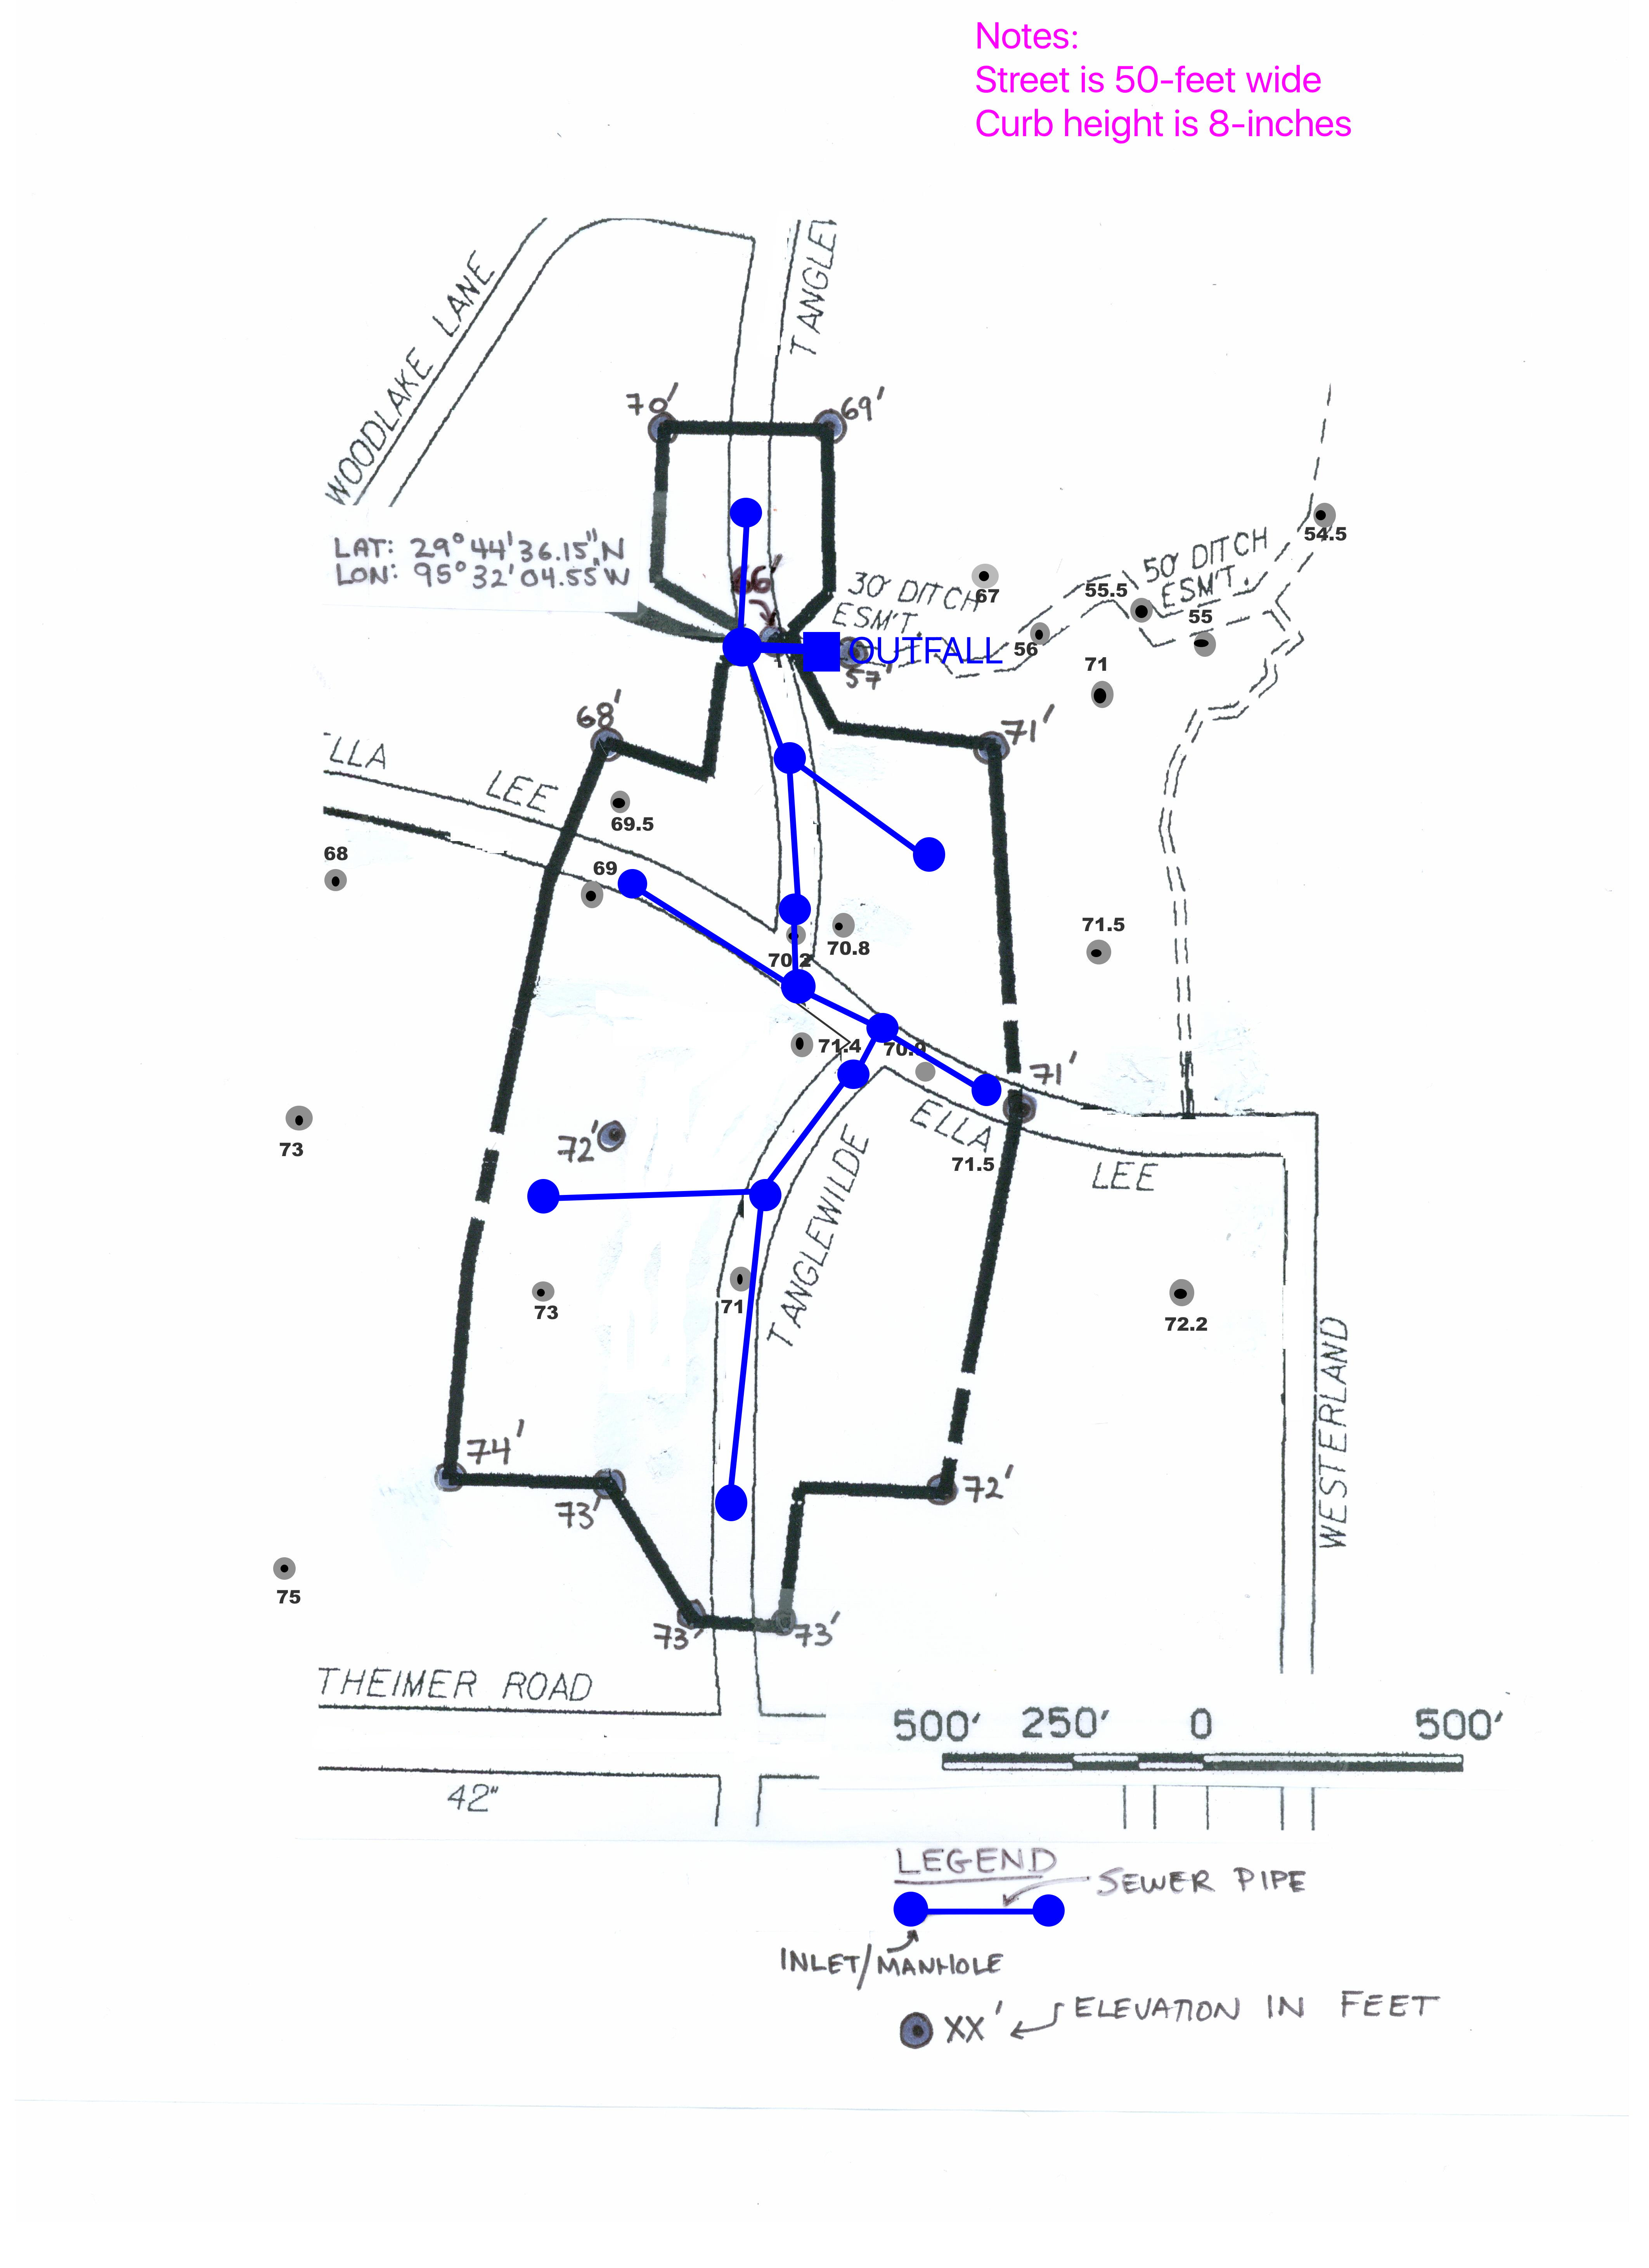
\includegraphics[height=7in]{Image119B.jpg} 
%   \caption{Tanglewilde Drive Storm Drain Inlet and Pipe Alignments}
%   \label{fig:survey}
%\end{figure}

%The figure shows land surface elevations in feet at the indicated locations.  
%A linear scale is shown in the legend.  
%Use the map(s) and:


%\clearpage
%
%\begin{enumerate}
%\item Construct a contour map of the area.
%Use the contour map determine the drainage areas to each inlet node.  
%Indicate which nodes you do not assign drainage (junction nodes for connecting pipes).
%\item Use the rational design method to size the conduits for a 5-year storm, for Harris County, Texas.
%\item Specify the invert (flow line) elevations of the nodes (inlets and junction boxes).
%\item Specify the soffit (crown) elevations for the pipes at each node.
%%\item Construct a SWMM model of the storm sewer system you just designed.   
%%Adjust the width of each drainage area so that the rational method is approximated in SWMM for each inlet, then apply a 3-hour, 5-year storm to the project.  
%%Specify the outlet as a free outfall, with the invert elevation as the bottom of the ditch.
%\end{enumerate}
%
%Submit a memorandum with screen captures of the relevant components above.













 









\end{document}  